\chapter[Uncertainty in SDM]{Uncertainty in Species Distribution Modeling}

\begin{objetivos}
By the end of this chapter, readers should be able to identify major sources of uncertainty in SDM; distinguish uncertainty from variability, model disagreement, environmental novelty, and systematic bias; examine contributions from occurrence data, predictors, calibration design, algorithms, global climate models, scenarios, extrapolation, and spatial scale; map algorithmic disagreement for \textit{Dinizia excelsa}; summarize variation across conditional projections without conflating it with probability; combine heterogeneous indicators transparently; and communicate SDM results critically and reproducibly.
\end{objetivos}

\section{Introduction}

Species distribution models do not produce absolute truths about species distributions. They produce estimates conditional on occurrence records, environmental predictors, the accessible area, sampling design, algorithm, parameterization, evaluation scheme, climate period, and projection scenario. A robust SDM analysis must therefore characterize the limitations and uncertainties relevant to its intended inference \parencite{guisan2017habitat,franklin2023,zurell2020benchmarking,yates2018transferability}.

For \textit{Dinizia excelsa}, this task is particularly important because the workflow combines potentially biased records of a large Amazonian tree, several correlative algorithms, climate surfaces, future projections, paleoclimate reconstructions, and temporal extrapolation. Agreement among outputs cannot repair a bias shared by all of these inputs.

\begin{conceito}[title={\faBook\quad Uncertainty in SDM}]
Uncertainty is incomplete knowledge about an estimate, process, or outcome. It may be represented by a probability distribution, interval, sensitivity analysis, disagreement surface, or qualitative limitation. Variability is observed or modeled heterogeneity; bias is systematic deviation; and environmental novelty measures departure from the calibration domain. These concepts are related but not interchangeable.
\end{conceito}

\section{An uncertainty taxonomy}

Useful categories include:

\begin{itemize}
\item \textbf{occurrence uncertainty}: identification errors, coordinate errors, temporal mismatch, imperfect detection, sampling bias, and limited sample size;
\item \textbf{predictor uncertainty}: measurement and interpolation error, product disagreement, scale mismatch, collinearity, and omission of relevant drivers;
\item \textbf{design uncertainty}: choices about the accessible area, background, thinning, folds, prevalence, and evaluation data;
\item \textbf{model uncertainty}: algorithm, feature representation, parameter values, tuning criterion, random seed, and fitted coefficients;
\item \textbf{projection uncertainty}: GCM, downscaling product, emissions pathway, time horizon, and paleoclimate reconstruction;
\item \textbf{transfer uncertainty}: environmental novelty, clamping, nonstationary relationships, dispersal, biotic interactions, and land-use change;
\item \textbf{decision uncertainty}: threshold, weighting, aggregation, utility, and the consequences assigned to false positives and false negatives.
\end{itemize}

Some components are reducible through better data or design; others reflect genuine variation among plausible futures or structural assumptions. A single map rarely captures them all.

\begin{atencao}[title={\faExclamationTriangle\quad Uncertainty is not disposable error}]
Uncertainty should not be hidden or treated as a defect that an ensemble automatically removes. It indicates where conclusions are stable, where they depend on analytical choices, and where additional evidence would be most valuable.
\end{atencao}

\section{Algorithmic disagreement}

Algorithmic disagreement describes variation among predictions from different modeling approaches. In this workflow, it is summarized by the cellwise standard deviation across GLM, GAM, Random Forest, BRT, and Maxent predictions.

\rscriptfile{scripts/unidade16/01_estrutura_pastas.R}

\rscriptfile{scripts/unidade16/02_incerteza_algoritmica_atual.R}

\begin{figure}[H]
\centering
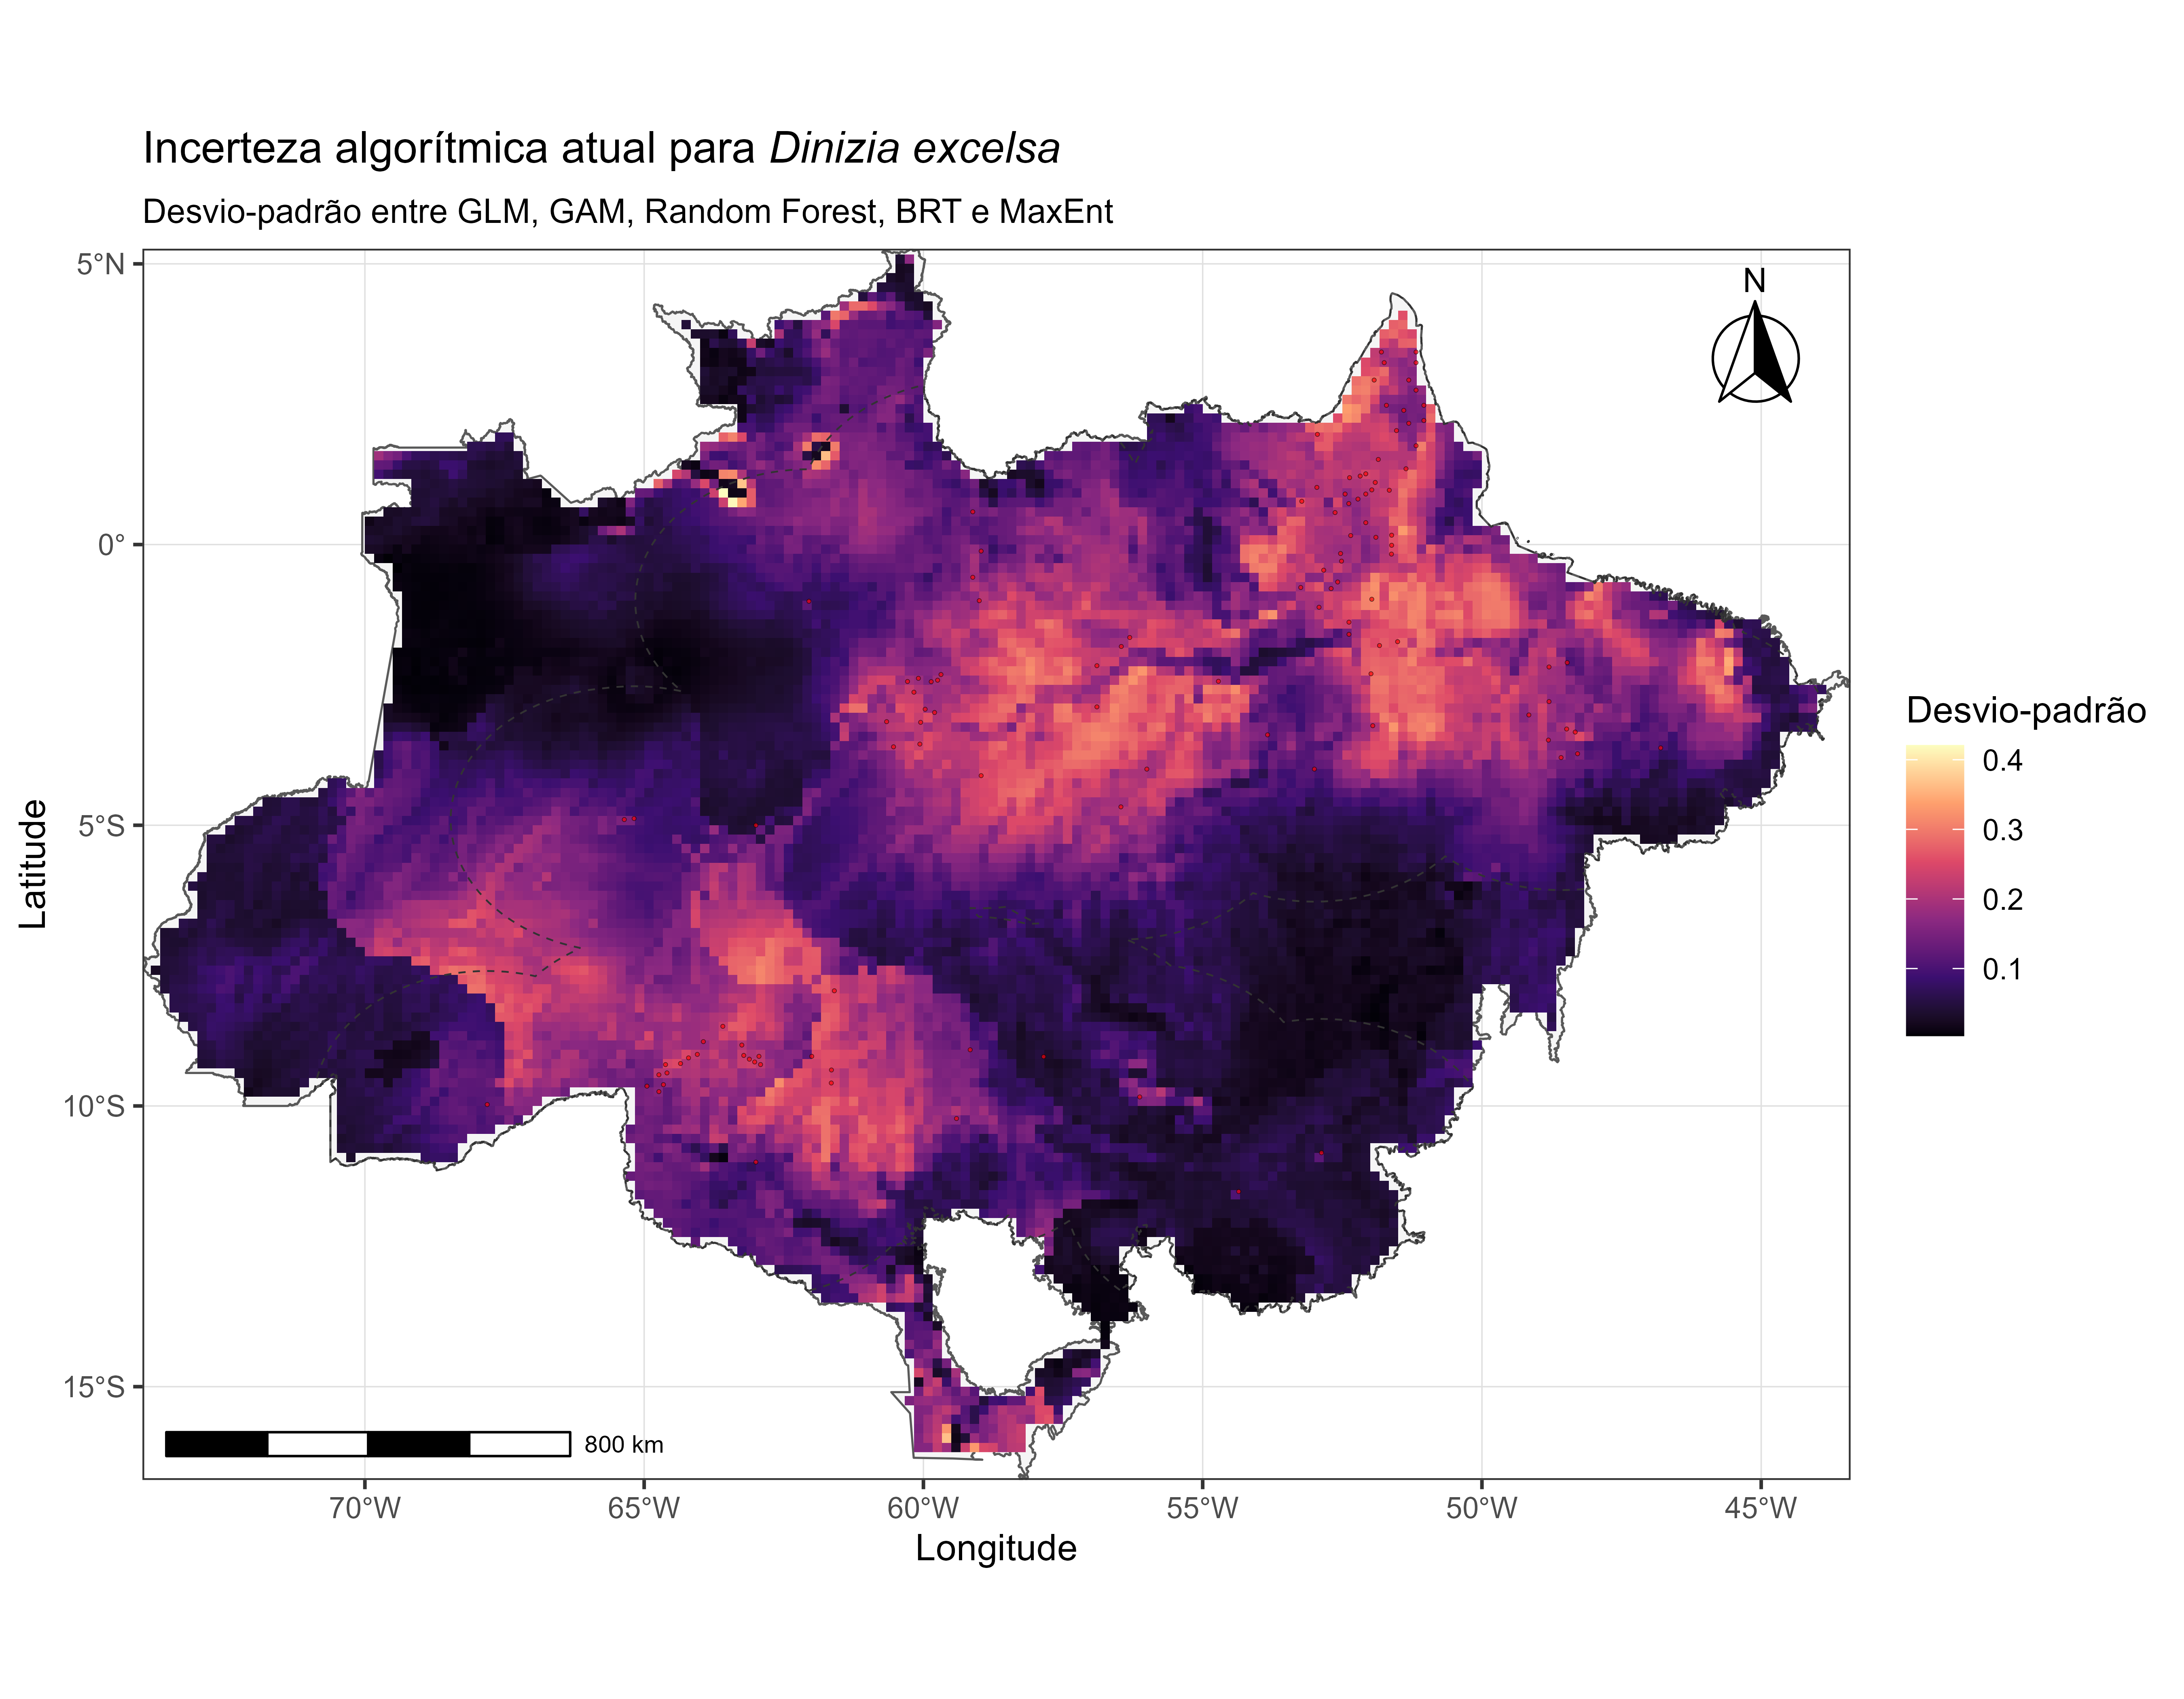
\includegraphics[width=0.88\textwidth]{figuras/unidade16/unidade16_incerteza_algoritmica_atual.png}
\caption{Contemporary algorithmic disagreement for \textit{Dinizia excelsa}, summarized by the standard deviation of predictions from GLM, GAM, Random Forest, BRT, and Maxent.}
\label{fig:unidade16_incerteza_algoritmica}
\end{figure}

This standard deviation is descriptive, not a confidence interval. Its interpretation is valid only when model outputs are on a sufficiently comparable scale. It also combines differences in algorithms with any differences in data subsets, tuning, or calibration procedures. To isolate algorithmic effects, keep other workflow components fixed and retain replicate or fold identifiers.

\section{Variation across future scenarios}

The spread among SSP1--2.6, SSP2--4.5, SSP3--7.0, and SSP5--8.5 projections describes sensitivity to alternative socioeconomic and forcing pathways. Because the pathways are conditional scenarios rather than random samples from a probability distribution, their standard deviation should not be interpreted as a probabilistic confidence measure.

\rscriptfile{scripts/unidade16/03_incerteza_cenarios_futuros.R}

\begin{figure}[H]
\centering
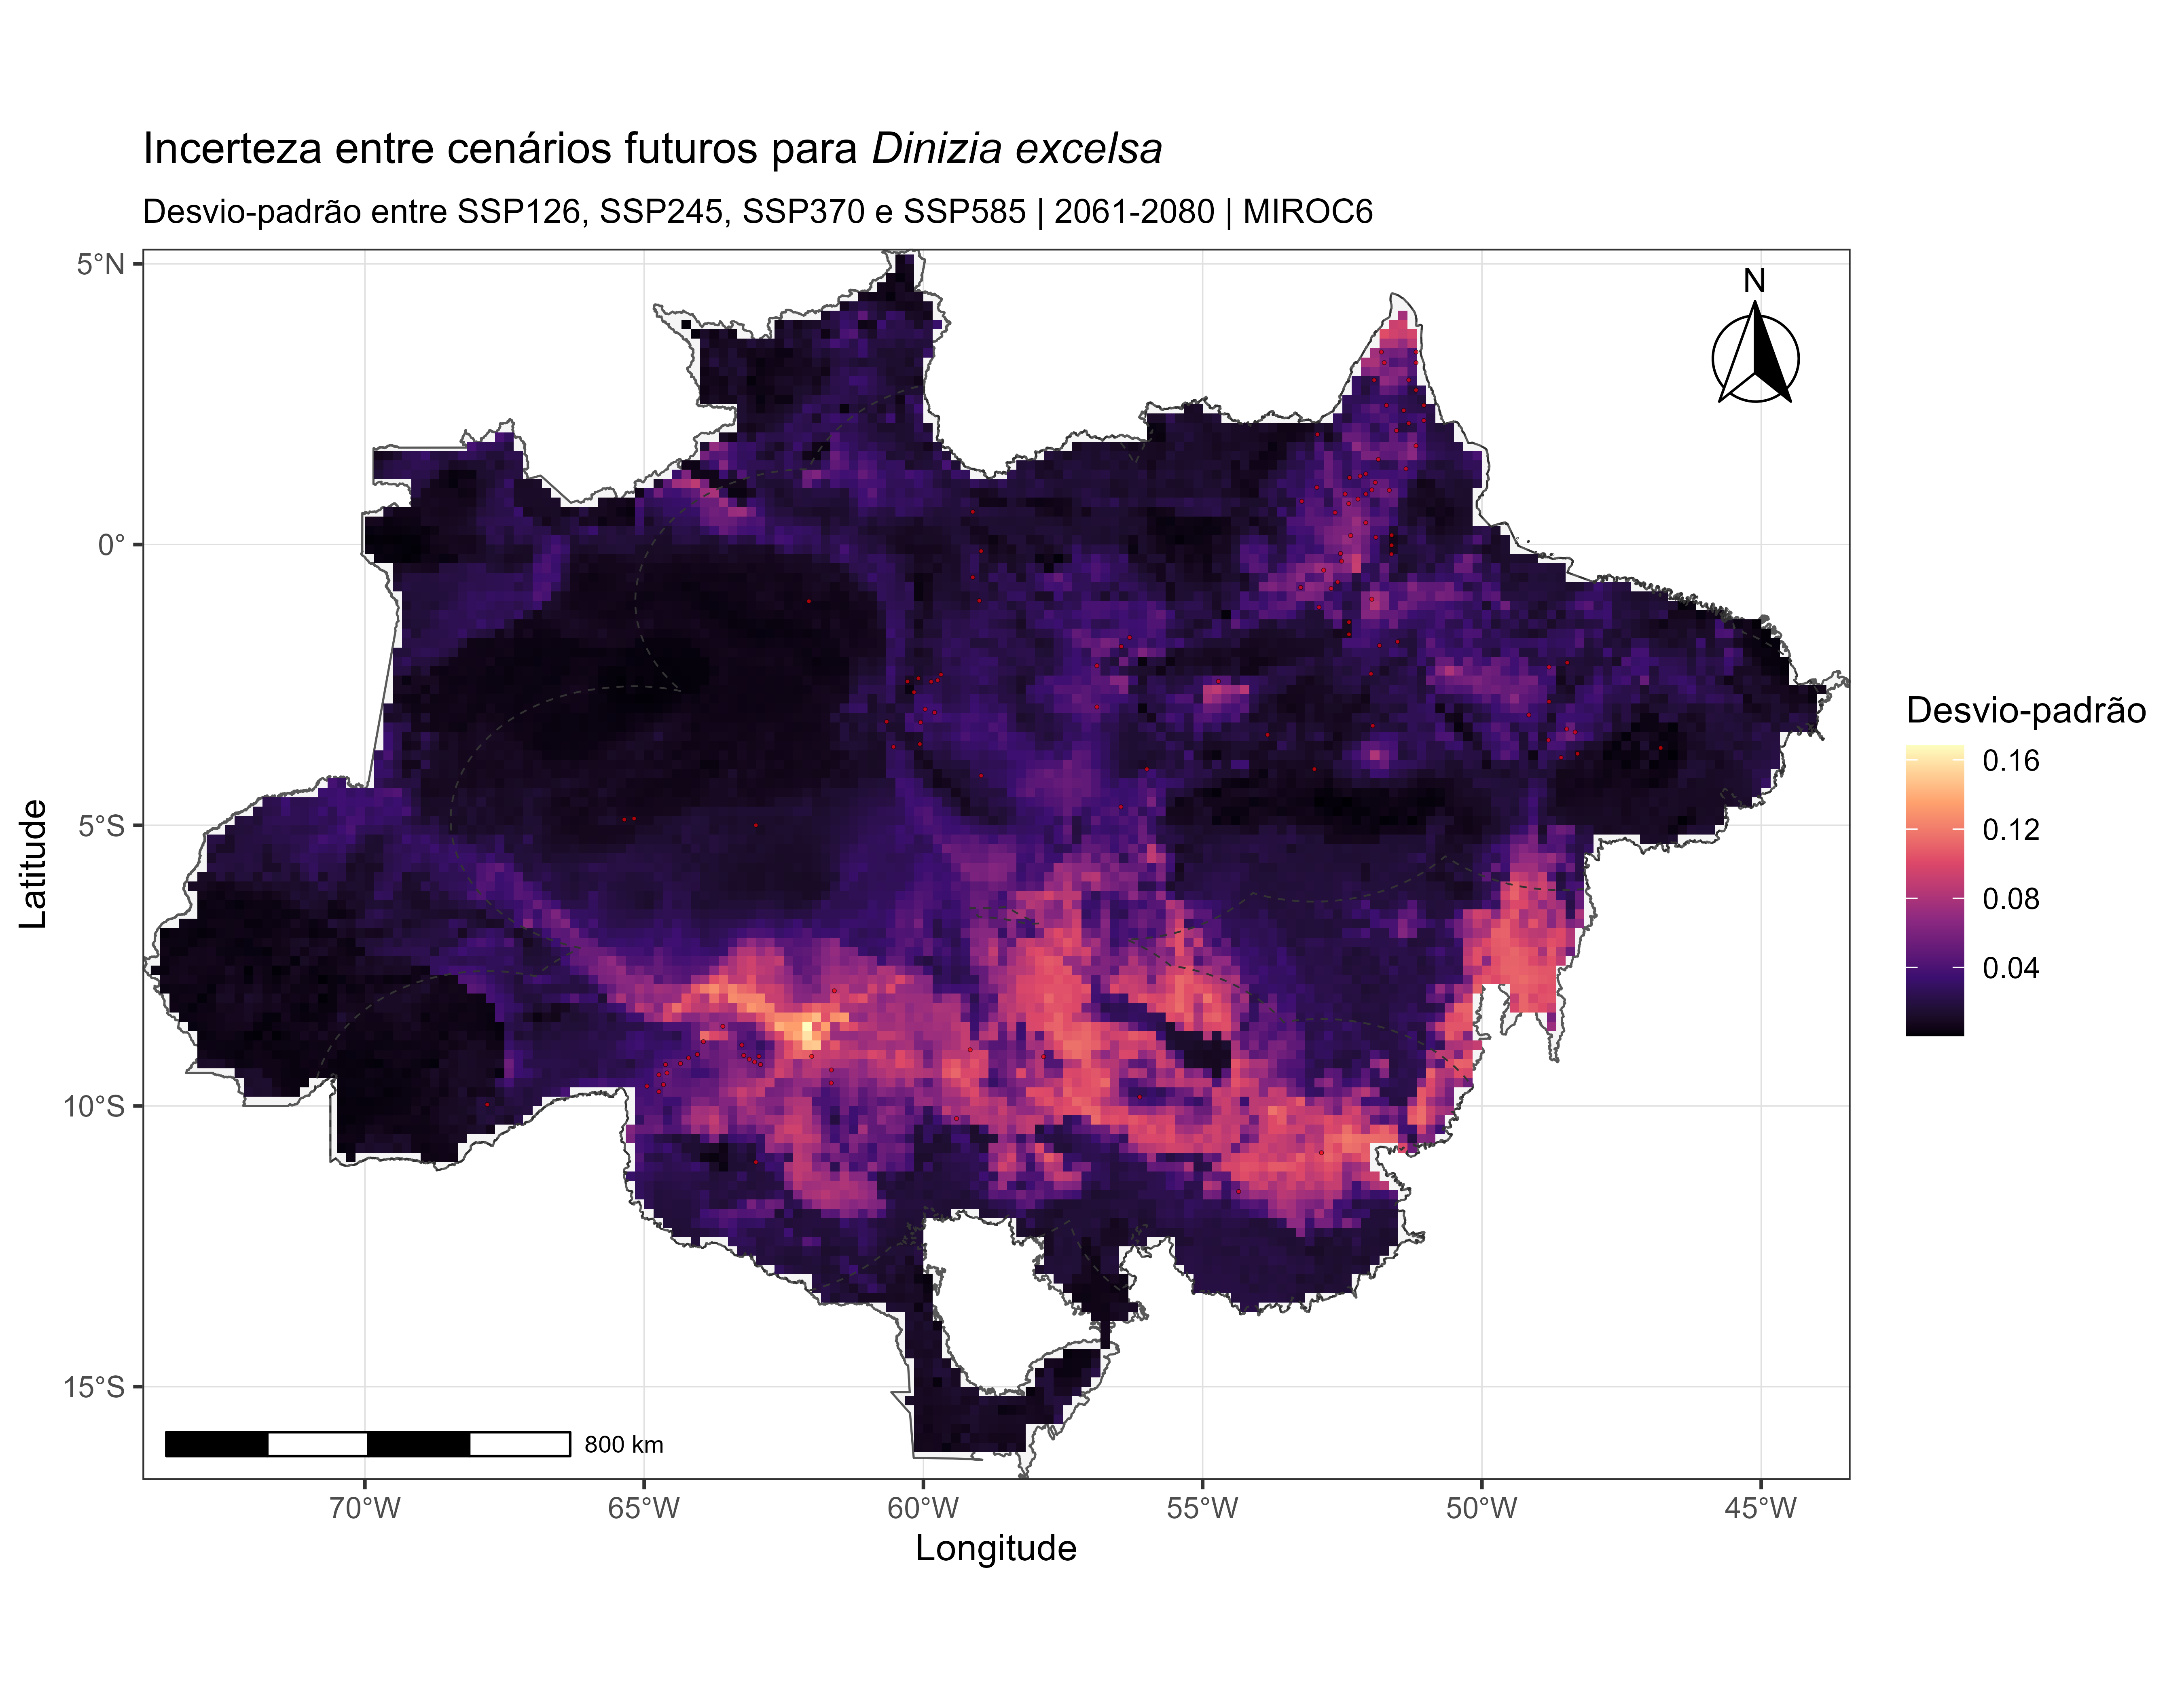
\includegraphics[width=0.88\textwidth]{figuras/unidade16/unidade16_incerteza_cenarios_futuros.png}
\caption{Spread among future ensemble projections for \textit{Dinizia excelsa} under SSP1--2.6, SSP2--4.5, SSP3--7.0, and SSP5--8.5.}
\label{fig:unidade16_incerteza_cenarios}
\end{figure}

A fuller factorial design separates at least algorithm, GCM, SSP, time horizon, and calibration replicate. Variation among GCMs under the same SSP reflects climate-model disagreement, whereas variation among SSPs reflects alternative boundary conditions and increases with the time horizon. Pooling both into one standard deviation obscures their distinct meanings.

\section{Environmental novelty and extrapolation risk}

MESS and MOP identify projection environments that depart from the calibration domain. They do not estimate prediction error directly and should not be treated as posterior uncertainty. Instead, they are diagnostics of support: extrapolative cells rely more strongly on fitted response shapes, clamping rules, and assumptions of temporal or spatial stationarity.

\rscriptfile{scripts/unidade16/04_incerteza_extrapolacao.R}

\begin{figure}[H]
\centering
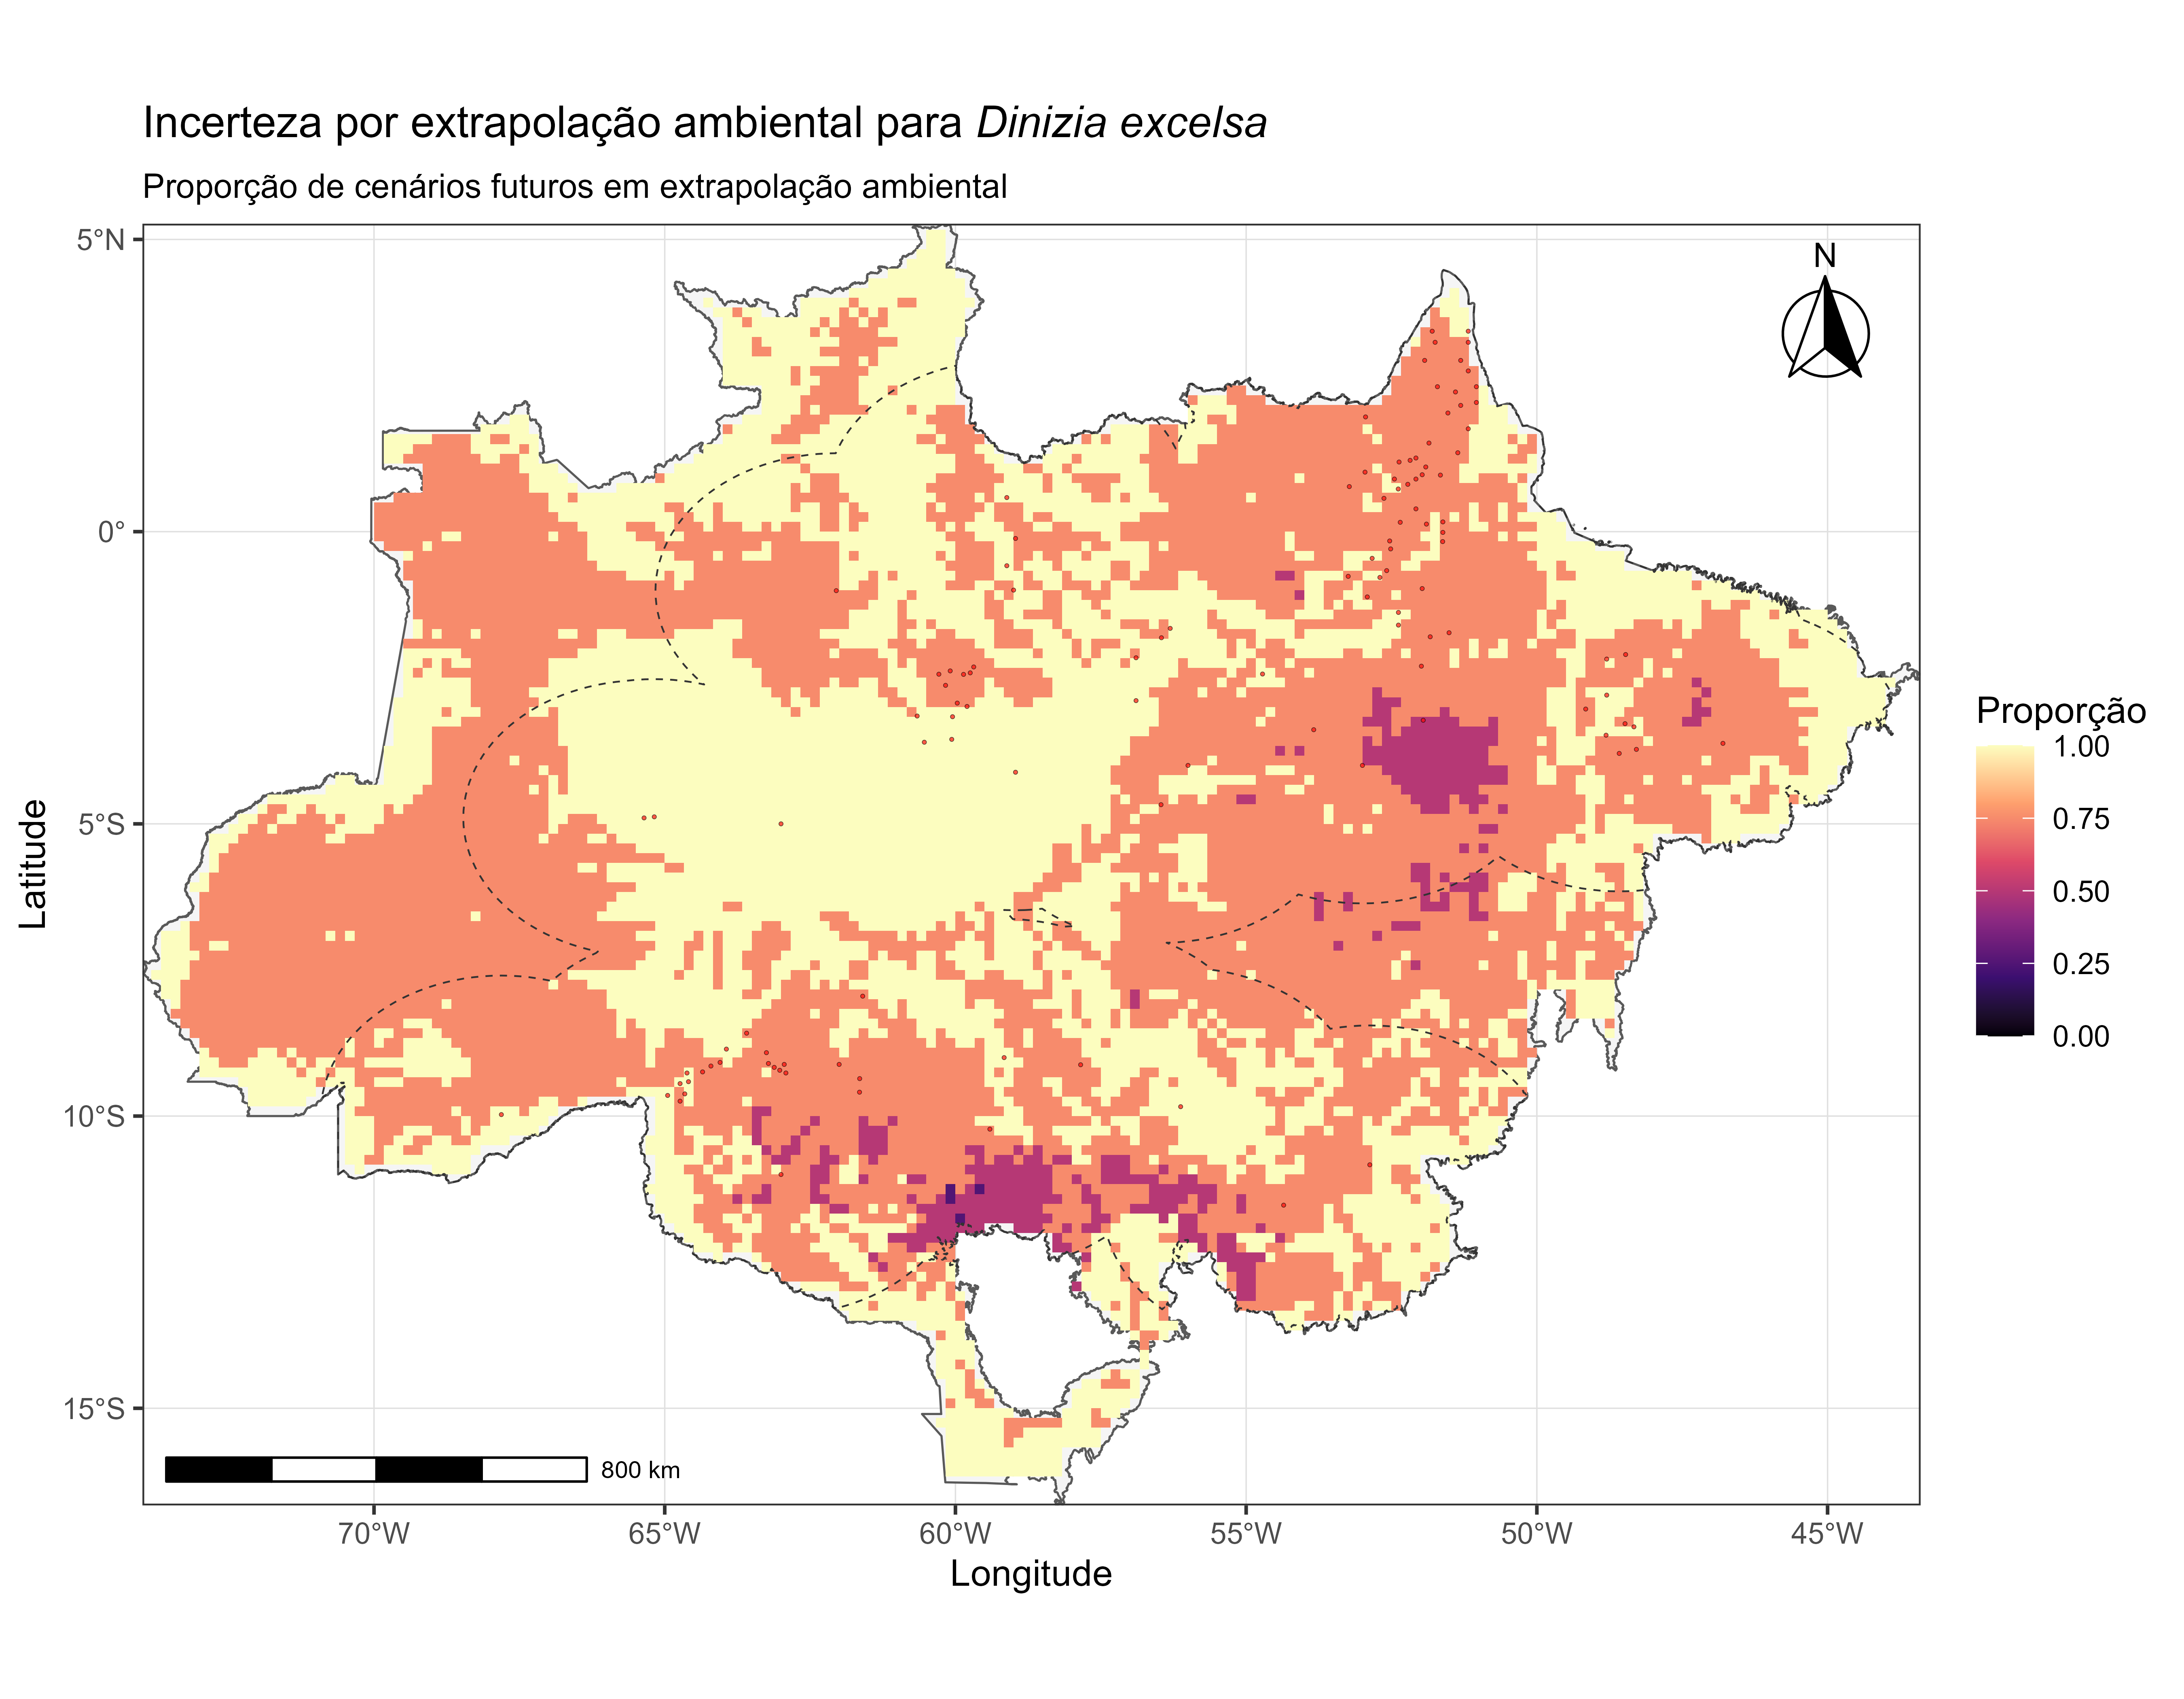
\includegraphics[width=0.96\textwidth]{figuras/unidade16/unidade16_incerteza_extrapolacao.png}
\caption{Environmental extrapolation risk in future projections for \textit{Dinizia excelsa}.}
\label{fig:unidade16_incerteza_extrapolacao}
\end{figure}

Novelty should therefore be reported alongside, rather than silently converted into, a prediction variance. A cell with low disagreement among algorithms can still be unsupported if all algorithms extrapolate similarly beyond the calibration data.

\section{Uncertainty in paleoclimate projections}

Paleoclimate applications include uncertainty from GCM structure, boundary conditions, downscaling, spatial resolution, reconstruction of past climates, predictor harmonization, and the assumption of niche conservatism. Uncertainty is best assessed by comparing alternative reconstructions for the same period and by propagating algorithmic and calibration variation within each reconstruction.

\rscriptfile{scripts/unidade16/05_incerteza_paleoclimatica.R}

\begin{figure}[H]
\centering
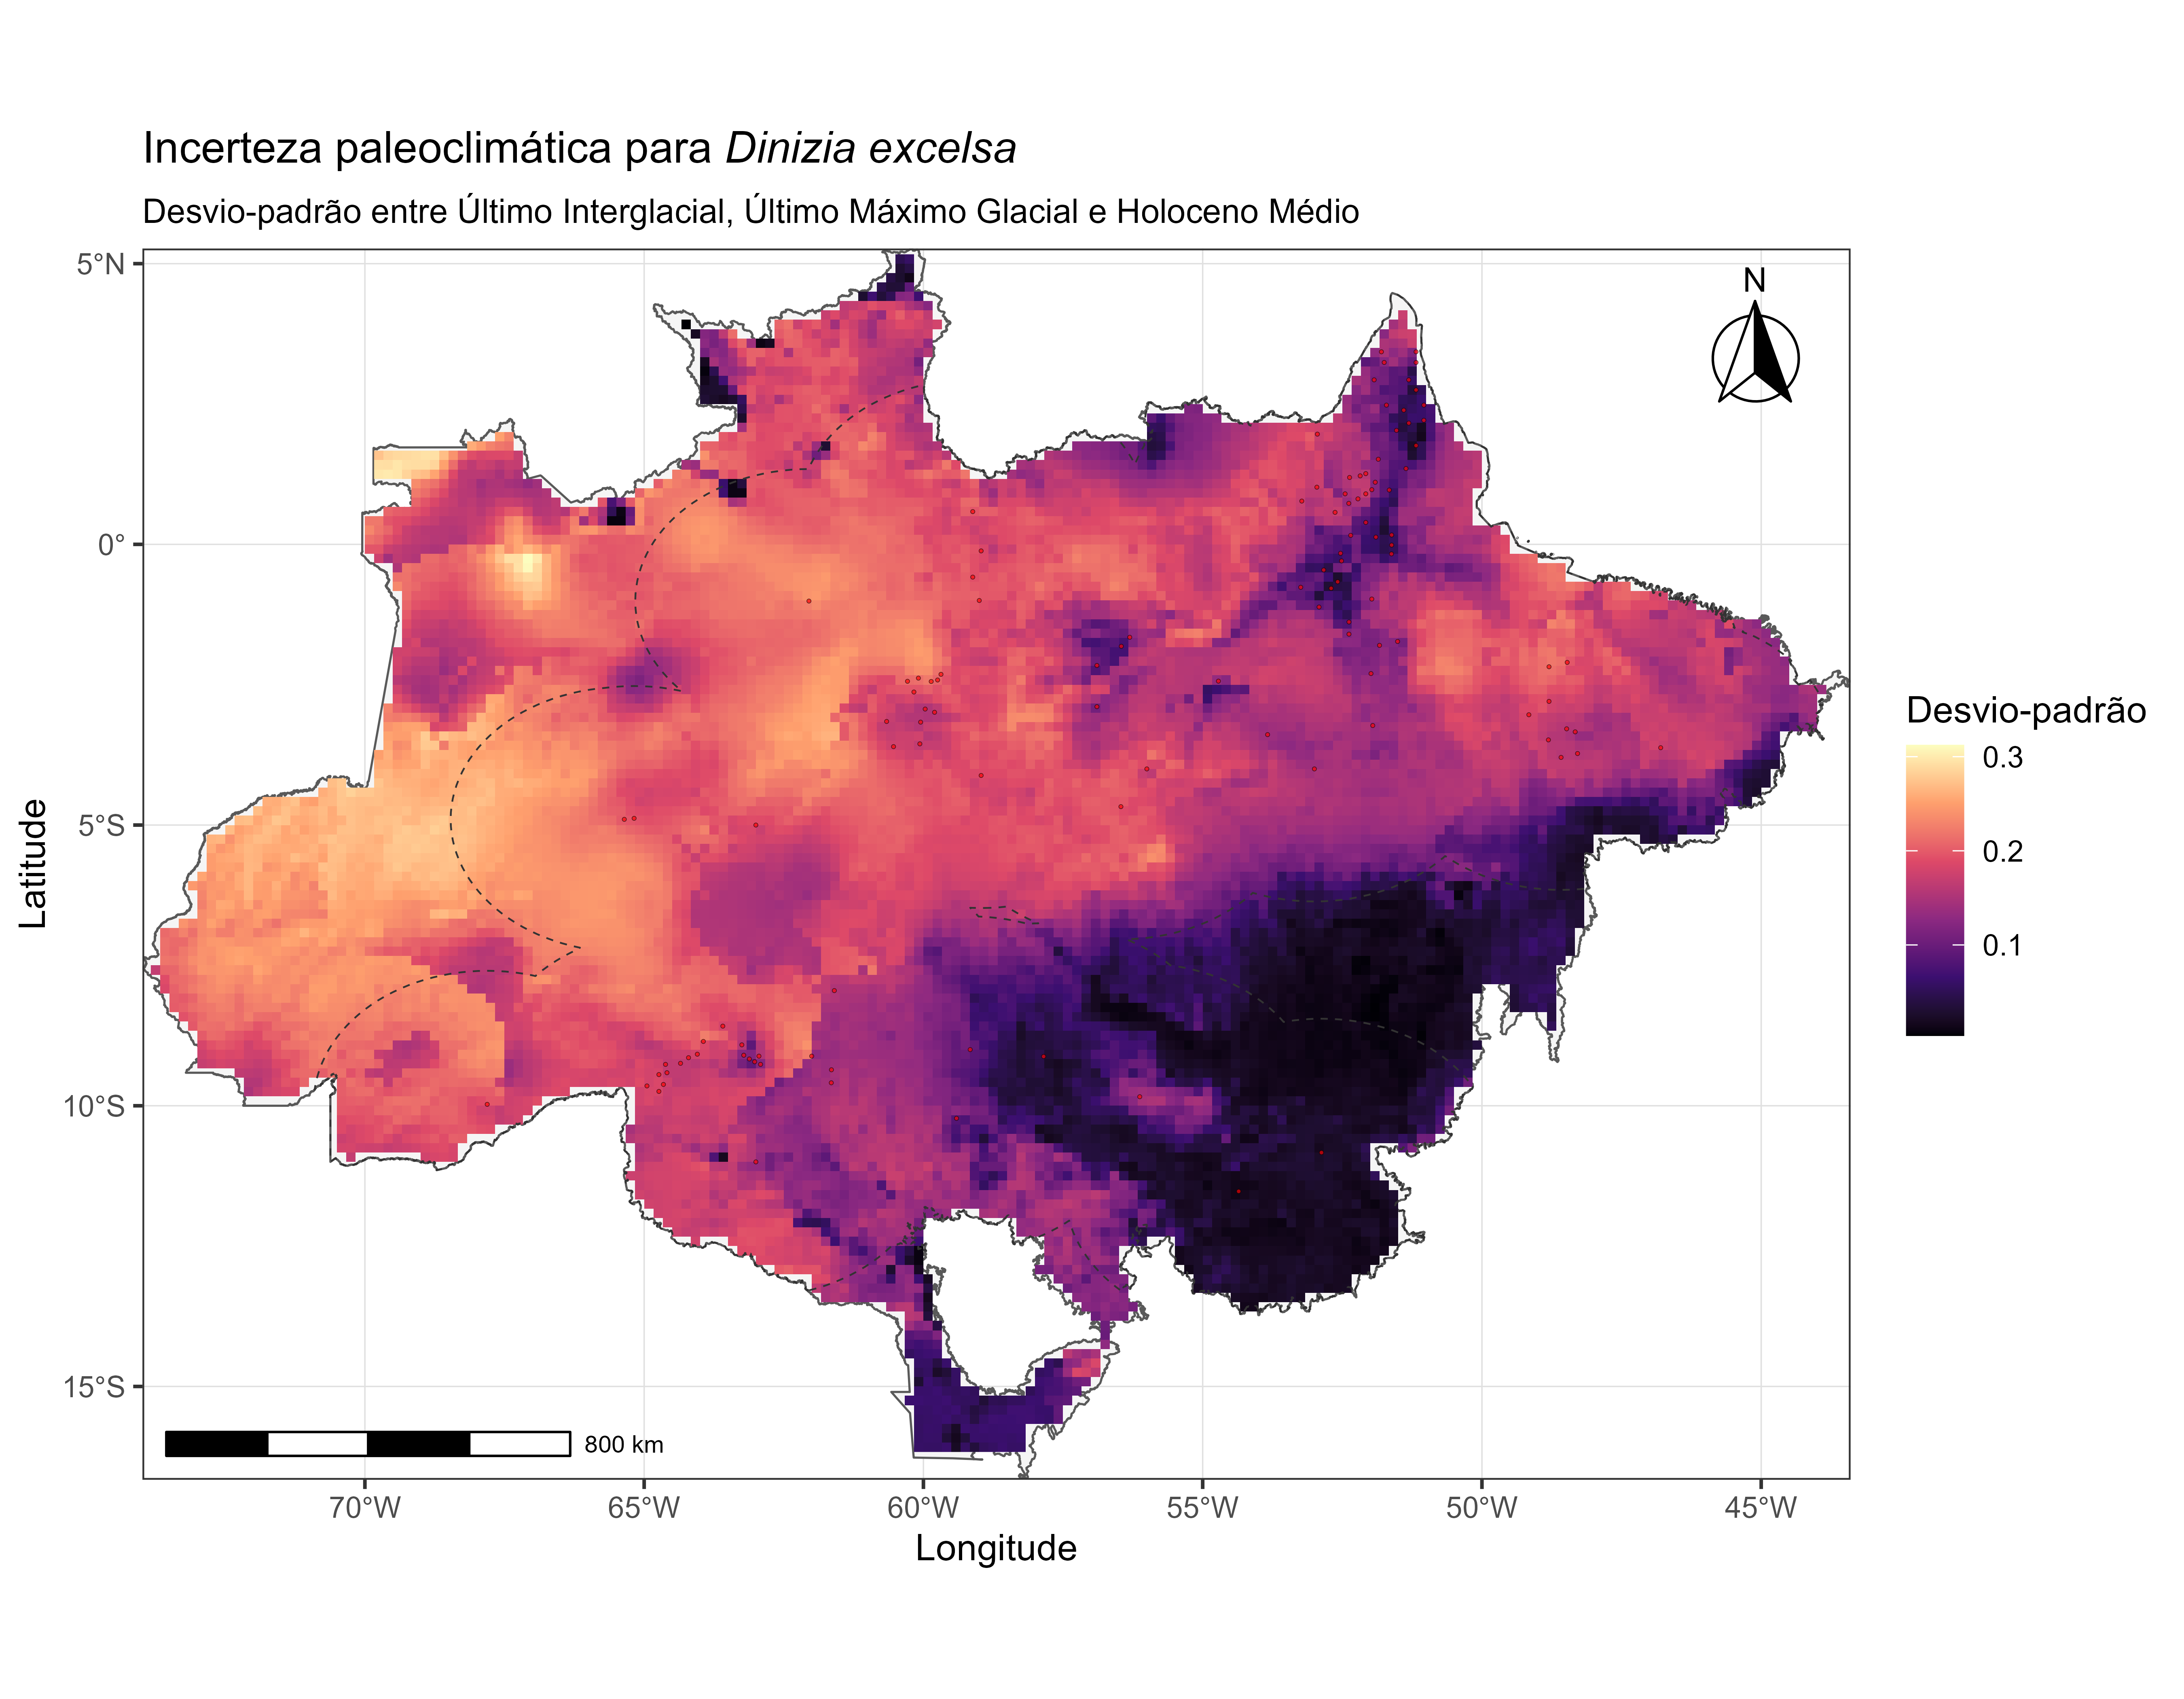
\includegraphics[width=0.88\textwidth]{figuras/unidade16/unidade16_incerteza_paleoclimatica.png}
\caption{Variation among paleoclimate projections for \textit{Dinizia excelsa}.}
\label{fig:unidade16_incerteza_paleo}
\end{figure}

Variation among the Last Interglacial, Last Glacial Maximum, and mid-Holocene is principally a temporal signal, not a replicate-based estimate of paleoclimate uncertainty. The workflow's cross-period map is useful as a stability diagnostic, but it should be labeled accordingly. A defensible uncertainty estimate would compare plausible GCMs or reconstructions within the same time slice.

\section{Integrated uncertainty indicators}

An integrated surface can summarize several diagnostics and highlight cells in which interpretation deserves caution.

\rscriptfile{scripts/unidade16/06_incerteza_integrada.R}

\begin{figure}[H]
\centering
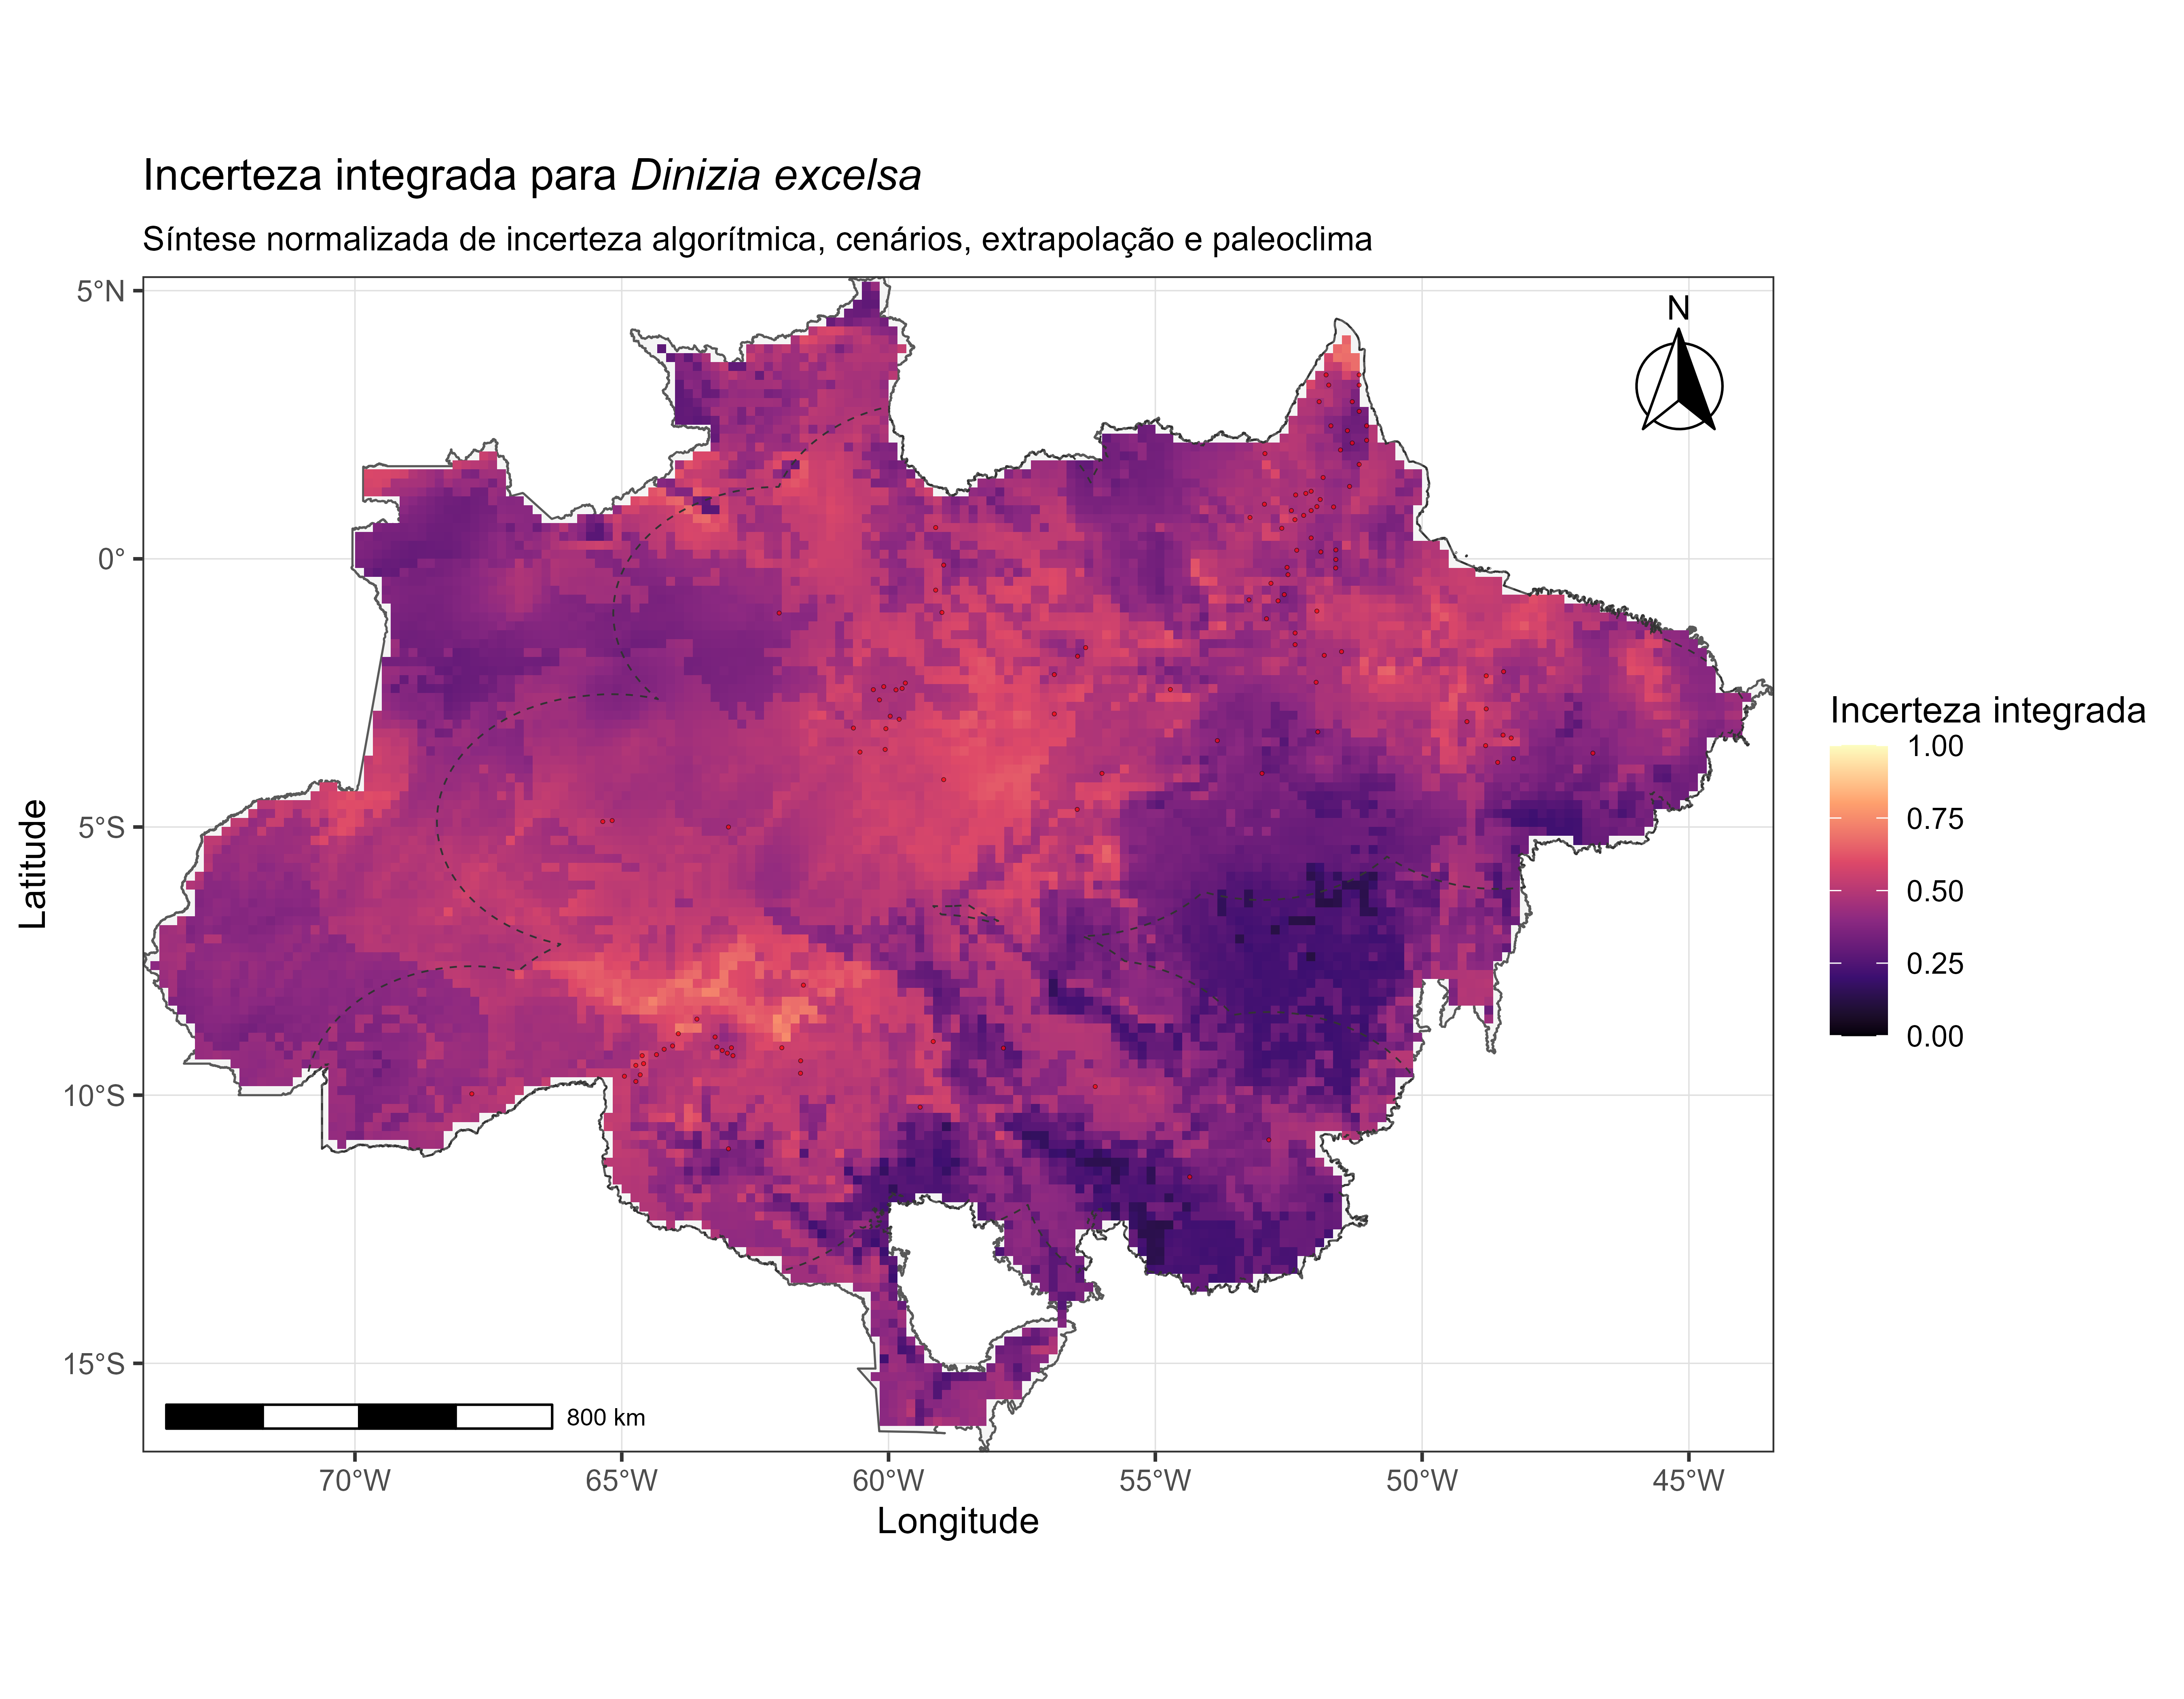
\includegraphics[width=0.88\textwidth]{figuras/unidade16/unidade16_incerteza_integrada.png}
\caption{Integrated caution index for \textit{Dinizia excelsa}, combining algorithmic disagreement, variation among future scenarios, environmental novelty, and paleoclimate variation.}
\label{fig:unidade16_incerteza_integrada}
\end{figure}

The combined surface should be called an \emph{index}, rather than a total variance, unless the components arise from a formally specified probabilistic model. Before aggregation, each component requires an explicit direction, scale, transformation, and weight. Normalizing all components to 0--1 makes them numerically combinable but does not make them conceptually equivalent. The unaggregated component maps must remain available so readers can see why a cell received a high index value.

\begin{atencao}[title={\faExclamationTriangle\quad Avoid double counting}]
Components may be dependent. Algorithmic spread can increase in novel environments, and scenario spread can include climate-model differences already summarized elsewhere. Adding correlated diagnostics can count the same source more than once. Document the dependency structure and test the sensitivity of the index to alternative weights.
\end{atencao}

\section{Suitability and uncertainty together}

Conservation interpretation benefits from considering predicted suitability and evidential support simultaneously. High-suitability, low-disagreement, environmentally analogous areas may represent relatively robust candidates. High-suitability areas with strong novelty or model disagreement are priority targets for verification, not automatically low-priority areas.

\rscriptfile{scripts/unidade16/07_adequabilidade_incerteza.R}

\begin{figure}[H]
\centering
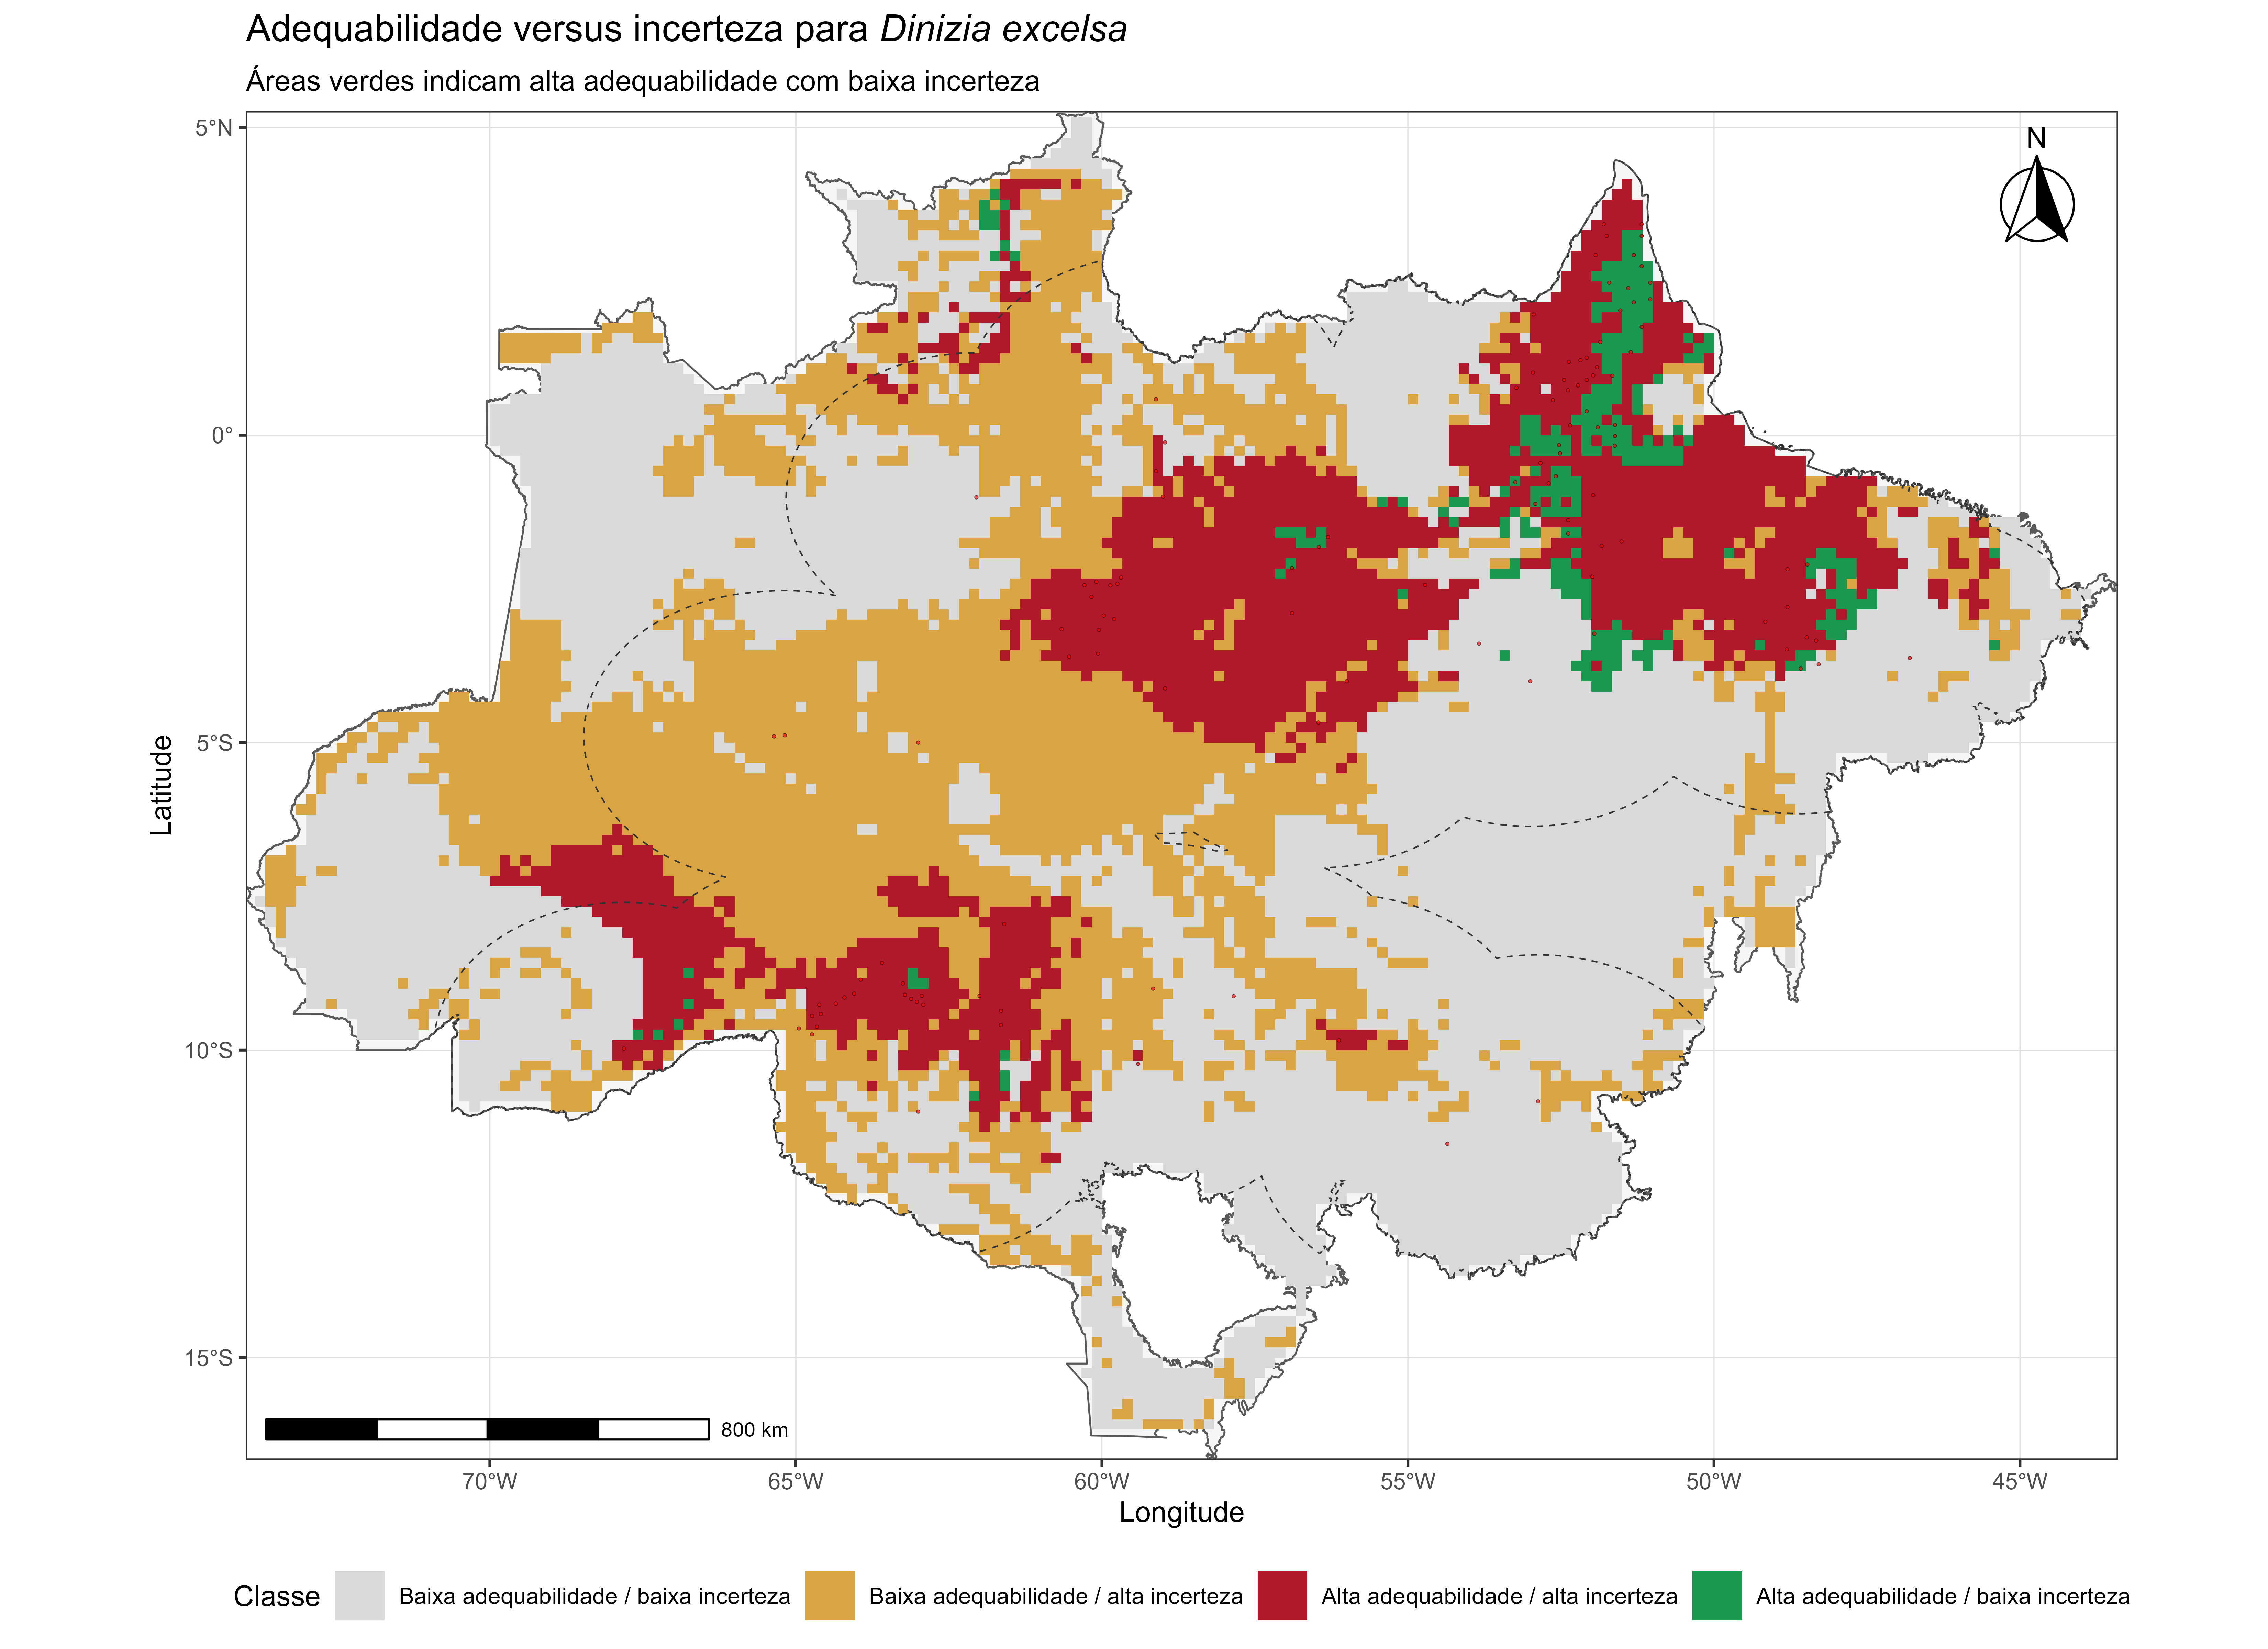
\includegraphics[width=0.96\textwidth]{figuras/unidade16/unidade16_adequabilidade_incerteza.png}
\caption{Joint classification of modeled suitability and the integrated uncertainty indicator for \textit{Dinizia excelsa}.}
\label{fig:unidade16_adequabilidade_incerteza}
\end{figure}

Classification cutoffs must be declared and subjected to sensitivity analysis. A high-versus-low matrix is a communication device and should not replace continuous surfaces, component diagnostics, or decision-specific costs.

\section{Quantitative synthesis}

\rscriptfile{scripts/unidade16/08_sintese_incertezas.R}

\begin{figure}[H]
\centering
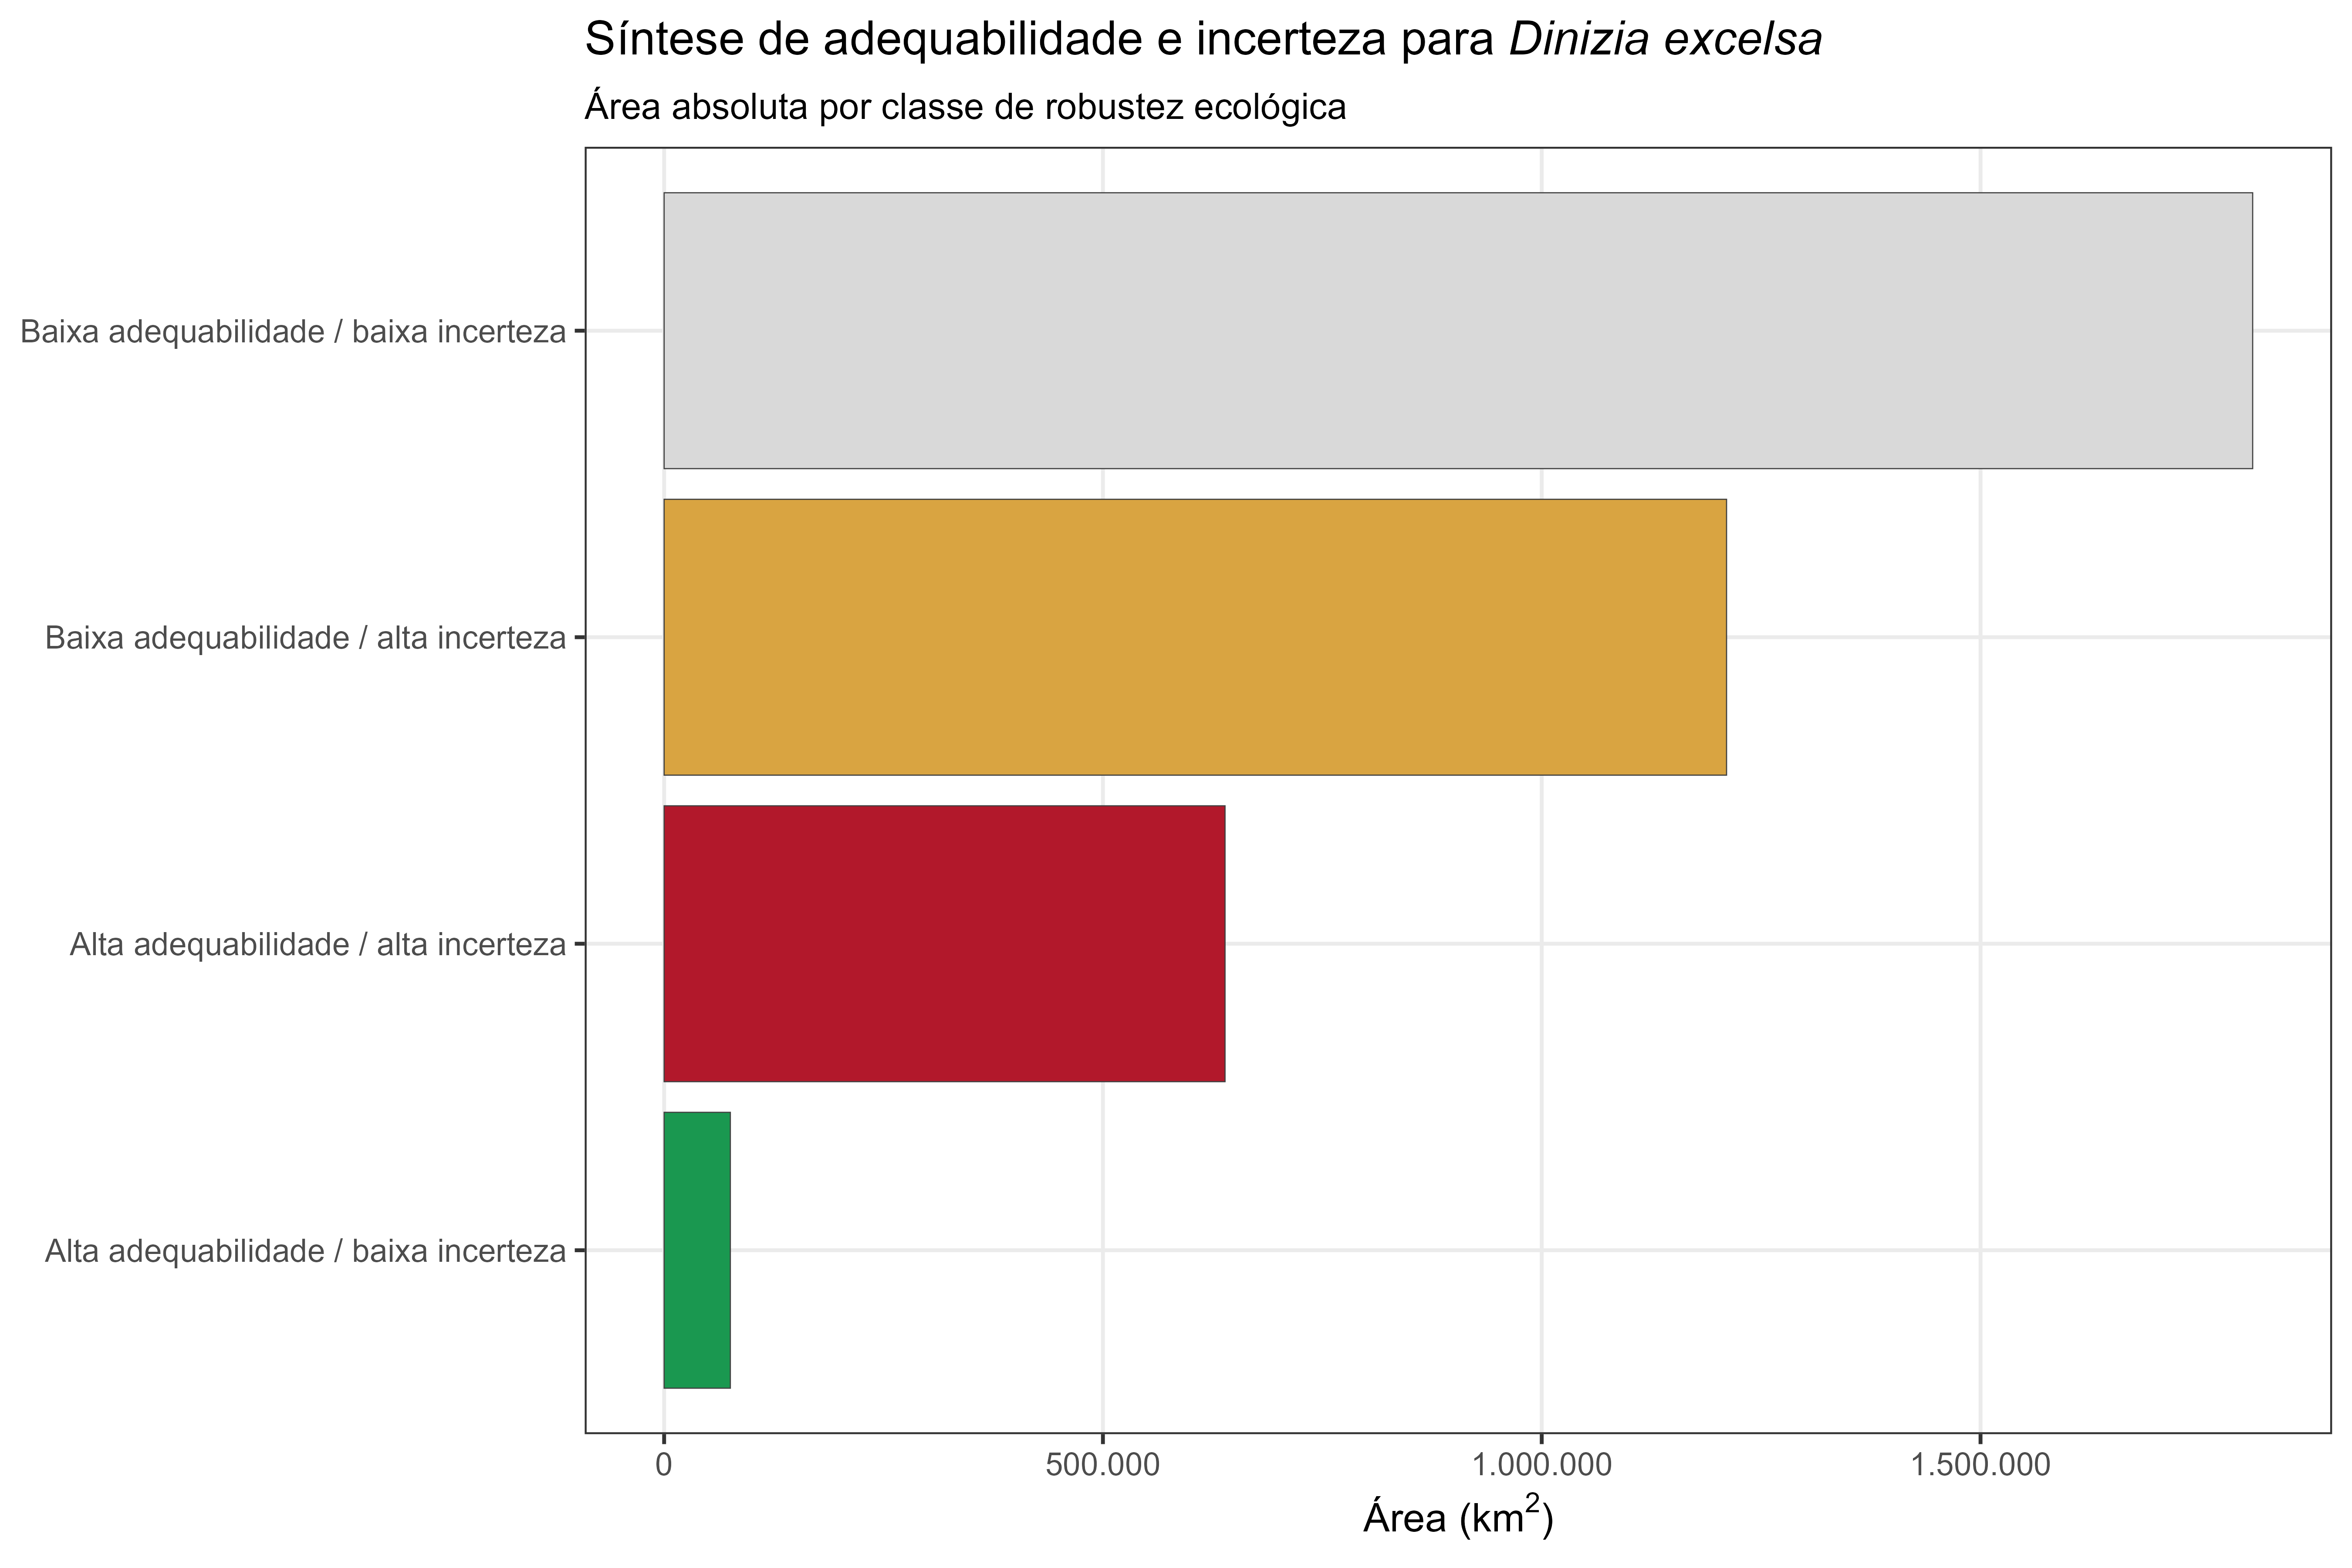
\includegraphics[width=0.88\textwidth]{figuras/unidade16/unidade16_sintese_incertezas.png}
\caption{Quantitative summary of joint suitability and uncertainty-index classes for \textit{Dinizia excelsa}.}
\label{fig:unidade16_sintese}
\end{figure}

Useful reporting includes maps and distributions for each component, factorial summaries by model and scenario, agreement on the sign of change, threshold sensitivity, and the proportion of the decision area supported by analogous environments. Where computationally feasible, resampling occurrences and calibration folds helps propagate sampling and estimation uncertainty.

\section{Complete pipeline}

\rscriptfile{scripts/unidade16/09_pipeline_incertezas.R}

\section{Chapter synthesis}

Uncertainty analysis turns SDM from a single cartographic product into a more transparent inferential workflow. For \textit{Dinizia excelsa}, separating algorithmic disagreement, conditional scenario variation, climate-model effects, paleoclimate reconstruction, and environmental novelty clarifies which conclusions are stable and which remain hypotheses.

\begin{conceito}[title={\faBook\quad Key message}]
Every SDM interpretation should ask two linked questions: what does the model estimate, and how strongly do the available data and assumptions support that estimate? No single standard-deviation map answers the second question completely.
\end{conceito}

\section{Review exercises}

\begin{enumerate}
\item Distinguish uncertainty, variability, disagreement, novelty, and bias using SDM examples.
\item What does the cellwise standard deviation among algorithms measure, and why is it not a confidence interval?
\item Why is variation among SSPs not automatically a probabilistic estimate of uncertainty?
\item How do MESS and MOP inform evidential support without directly measuring prediction error?
\item Why is variation among different paleoclimatic periods a temporal signal rather than a pure uncertainty estimate?
\item How should high suitability combined with high novelty or disagreement be interpreted?
\item What information must accompany an integrated uncertainty index used in conservation planning?
\end{enumerate}

